%PREAMBLE
\begin{comment}
%\documentclass[11pt]{article}
%\newcommand{\pablo}[1]{\textcolor{blue}{{\bf  #1}}}
\newcommand{\carlos}[1]{\textcolor{red}{{\bf  #1}}}
\newcommand{\fabio}[1]{\textcolor{purple}{{\bf  #1}}}
\newcommand{\susana}[1]{\textcolor{violet}{{\bf  #1}}}

% HEP names :: https://ctan.javinator9889.com/macros/latex/contrib/hepnames/hepnames.pdf

\DeclarePairedDelimiter\bra{\langle}{\rvert}
\DeclarePairedDelimiter\ket{\lvert}{\rangle}
\DeclarePairedDelimiterX\braket[2]{\langle}{\rangle}{#1 \delimsize\vert #2}

\newcommand*{\yt}{\ensuremath{y_{t}}\xspace}
\newcommand*{\tchannel}{\ensuremath{t\text{-channel}}\xspace}
\newcommand*{\schannel}{\ensuremath{s\text{-channel}}\xspace}
%\newcommand*{\lepT}{\ensuremath{\Pl_{\Pt}}\xspace}
%\newcommand*{\lepH}{\ensuremath{\Pl_{\PHiggs}}\xspace}

%\newcommand*{\muR}{\ensuremath{\mu_{\text{R}}}\xspace}
%\newcommand*{\muF}{\ensuremath{\mu_{\text{F}}}\xspace}

% Add external packages
\usepackage[italic]{hepnicenames}

%%%%%%%%%%%%%%%%%%%%%%%
%  From NA-HIGG-2020-02-INT1-defs.sty    %
%%%%%%%%%%%%%%%%%%%%%%%
% Basic tHq-related macros
%\newcommand*{\tHq}{\ensuremath{\Pqt{}\PH{}\Pq}\xspace}
%\newcommand*{\tHq}{\ensuremath{\Ptop \PHiggs \Pq}\xspace}
%\newcommand*{\tHq}{\Pqt{}\PH{}\Pq}
\newcommand*{\tHq}{\ensuremath{tHq}\xspace}
\newcommand*{\tH}{\ensuremath{\Pqt{}\PH{}}\xspace}
\newcommand*{\tHqsec}{\texorpdfstring{\Pqt{}\PH{}\Pq}{tHq}}
\newcommand*{\tHqML}{\ensuremath{\Pqt{}\PH{}\Pq\,(\text{ML})}\xspace}
\newcommand*{\tHqbb}{\ensuremath{\Pqt{}\PH{}\Pq\,(\bbbar)}\xspace}
\newcommand*{\tbarHq}{\Paqt{}\PH{}Pq}
\newcommand*{\tHbb}{\ensuremath{\tHq (\PH \to \bbbar)}\xspace}
\newcommand*{\tHtautau}{\ensuremath{\tHq (\PH \to \Pgt{}\Pgt)}\xspace}
\newcommand*{\dR}{\ensuremath{\Delta R}\xspace}
\newcommand*{\trexfitter}{TRExFitter\xspace}
\newcommand*{\thqloop}{\texttt{tHqLoop}\xspace}


\newcommand*{\MpT}{\ensuremath{\vec{p}_{\text{T}}^{\text{miss}}}\xspace}
\newcommand*{\mtw}{\ensuremath{m_{\text{T}}(\Pl,\MET)}}
\newcommand*{\mlb}{\ensuremath{m_{\Pl\Pqb}}}
\newcommand*{\mOSSF}{\ensuremath{m_{\text{OSSF}}}\xspace}

% Background processes
\newcommand*{\ttX}{\ensuremath{\Pqt{}\Paqt{}X}\xspace}
\newcommand*{\tX}{\ensuremath{\Pqt{}X}\xspace}

%\newcommand*{\ttX}{\Pqt{}\Paqt{}+X}
\newcommand*{\ttH}{\Pqt{}\Paqt{}\PH}
%\newcommand*{\ttH}{\ensuremath{\Pqt{}\Paqt{}\PH}\xspace}
\newcommand*{\ttZ}{\Pqt{}\Paqt{}\PZ}
\newcommand*{\ttV}{\ensuremath{\Pqt{}\Paqt{}V}\xspace}
\newcommand*{\ttW}{\Pqt{}\Paqt{}\PW}
\newcommand*{\ttWj}{\ensuremath{t\bar{t}W+j}\xspace}
\newcommand*{\tZq}{\Pqt{}\PZ{}\Pq}
\newcommand*{\tWZ}{\Pqt{}\PW{}\PZ}
\newcommand*{\tWH}{\Pqt{}\PW{}\PH}
\newcommand*{\tHW}{\Pqt{}\PW{}\PH}
\newcommand*{\tW}{\Pqt{}\PW}
\newcommand*{\Wt}{\Pqt{}\PW}
\newcommand*{\diboson}{diboson\xspace}
\newcommand*{\Diboson}{Diboson\xspace}
\newcommand*{\triboson}{triboson\xspace}
\newcommand*{\Triboson}{Triboson\xspace}
\newcommand*{\Vjets}{\ensuremath{V\text{+\,jets}}\xspace}

\newcommand*{\ttt}{\ensuremath{ttt}\xspace}
\newcommand*{\tttt}{\ensuremath{t\bar{t}t\bar{t}}\xspace}
\newcommand*{\ggH}{\ensuremath{ggH}\xspace}
\newcommand*{\qqH}{\ensuremath{qqH}\xspace}
\newcommand*{\WH}{\ensuremath{WH}\xspace}
\newcommand*{\ZH}{\ensuremath{ZH}\xspace}

% Fake leptons
\newcommand*{\elHF}{\ensuremath{e_{\text{HF}}}\xspace}
\newcommand*{\muHF}{\ensuremath{\mu_{\text{HF}}}\xspace}
\newcommand*{\elCo}{\ensuremath{e_{\text{conv}}}\xspace} 
\newcommand*{\kelHF}{\ensuremath{\mu(e_{\text{HF}})}\xspace}
\newcommand*{\kmuHF}{\ensuremath{\mu(\mu_{\text{HF}})}\xspace}
\newcommand*{\kelCo}{\ensuremath{\mu(e_{\text{conv}})}\xspace} 

% Signal regions
\newcommand*{\dileptau}{\ensuremath{2\Pl+1\tauhad}\xspace}
\newcommand*{\dilepOStau}{\ensuremath{2\Pl\,\text{OS}+1\tauhad}\xspace}
\newcommand*{\dilepSStau}{\ensuremath{2\Pl\,\text{SS}+1\tauhad}\xspace}

\newcommand*{\onelep}{\ensuremath{1\Pl}\xspace}
\newcommand*{\dilep}{\ensuremath{2\Pl}\xspace}
\newcommand*{\dilepOS}{\ensuremath{2\Pl\,\text{OS}}\xspace}
\newcommand*{\dilepSS}{\ensuremath{2\Pl\,\text{SS}}\xspace}
%\newcommand*{\SS}{\ensuremath{\text{SS}}\xspace}
%\newcommand*{\OS}{\ensuremath{\text{OS}}\xspace}

\newcommand*{\trilep}{\ensuremath{3\Pl}\xspace}
\newcommand*{\lepditau}{\ensuremath{1\Pl+2\tauhad}\xspace}




\newcommand*{\lumi}{\ensuremath{\mathcal{L}}\xspace}
\newcommand*{\lumiunits}{$\,$ cm$^{2} \,$s$^{-1}$\xspace}


%Other
\newcommand*{\CM}{\ensuremath{\sqrt{s}}\xspace}
 
\newcommand*{\Wtb}{\ensuremath{tWb}\xspace}
\newcommand*{\tWb}{\Wtb}
%\newcommand*{\tWb}{\ensuremath{tWb}\xspace}
\newcommand*{\pfour}{\ensuremath{\boldsymbol{\textrm{p}}}\xspace} 

\newcommand*{\tchan}{\ensuremath{t}-channel}
\newcommand*{\mtop}{\ensuremath{m_{\Ptop}}\xspace}
%\newcommand*{\mH}{\ensuremath{m_H}\xspace}
%\newcommand*{\HT}{\ensuremath{H_{\text{T}}}\xspace}

%\newcommand*{\PWplus}{\ensuremath{\PW^{+}}\xspace}
%\newcommand*{\PWminus}{\ensuremath{\PW^{-}}\xspace}
%\newcommand*{\Pgamma}{\ensuremath{\gamma}\xspace}

 \newcommand*{\greekphys}{\ensuremath{\varphi\upsilon\sigma\iota\kappa \eta}\xspace}
 \newcommand*{\greekatom}{\ensuremath{\alpha \tau o \mu o \nu}\xspace}
 \newcommand{\emu}{\ensuremath{\Pe/\Pmu}\xspace}

\newcommand*{\momentum}{\ensuremath{\overrightarrow{p}}\xspace} 
%\newcommand*{\CP}{\ensuremath{\mathcal{CP}}\xspace}
\newcommand*{\CP}{CP\xspace}

% Decays (Please, check latex/atlasprocess.sty and latex/atlasparticle.sty for more definitions!)
\newcommand{\bb}{\ensuremath{\Pqb\Paqp}\xspace}
\newcommand{\WW}{\ensuremath{\PW\PW^{*}}\xspace}
\newcommand{\ZZ}{\ensuremath{\PZ\PZ^{*}}\xspace}
\newcommand{\Higgsdecays}{\ensuremath{\PH \rightarrow b\bar{b}, \WW, \ZZ, \tau\tau}\xspace}
\newcommand{\Higgsdecayslep}{\ensuremath{\PH \rightarrow \WW, \ZZ, \tau\tau}\xspace}
\newcommand{\HWW}{\ensuremath{\PH \rightarrow \WW}\xspace}
\newcommand{\HZZ}{\ensuremath{\PH \rightarrow \ZZ}\xspace}

% reconstruction definitions
\newcommand{\pnutop}{\ensuremath{\vec{p^{\Pnu, \text{top}}}}\xspace}
\newcommand{\pnutopx}{\ensuremath{p^{\Pnu, \text{top}}_x}\xspace}
\newcommand{\pnutopy}{\ensuremath{p^{\Pnu, \text{top}}_y}\xspace}
\newcommand{\pnutopz}{\ensuremath{p_{z}(\Pnu_{\text{top}})}\xspace}
\newcommand{\pnutopT}{\ensuremath{\pT(\Pnu_{\text{top}})}\xspace}
\newcommand{\phinutop}{\ensuremath{\phi(\Pnu_{\text{top}})}\xspace}
\newcommand{\pltop}{\ensuremath{\vec{p^{\Plepton, \text{top}}}}\xspace}
\newcommand{\pltopx}{\ensuremath{p^{\Plepton, \text{top}}_x}\xspace}
\newcommand{\pltopy}{\ensuremath{p^{\Plepton, \text{top}}_y}\xspace}
\newcommand{\pltopz}{\ensuremath{p^{\Plepton, \text{top}}_z}\xspace}
\newcommand{\pltopT}{\ensuremath{\pT(\Plepton_{\text{top}})}\xspace}
\newcommand{\philtop}{\ensuremath{\phi(\ell_{\text{top}})}\xspace}
\newcommand{\phibtop}{\ensuremath{\phi(b_{\text{top}})}\xspace}
\newcommand{\tauvis}{\ensuremath{\Ptau_{\text{vis}}}\xspace}

\newcommand{\leptop}{\ensuremath{\Plepton^{\text{top}}}\xspace}
\newcommand{\lepH}{\ensuremath{{\Plepton^{\PH}}}\xspace}
\newcommand{\Hvismass}{\ensuremath{m_{\PH}^{\text{vis}}}\xspace}
\newcommand{\toprecomass}{\ensuremath{\mtop^{\text{reco}}}\xspace}
% \newcommand{\toprecomass}{\ensuremath{\Pqt_{\text{reco}}^{\text{m}}\xspace}}
% \newcommand{\Hvismass}{\ensuremath{\PH_{\text{vis}}^{\text{m}}\xspace}}
\newcommand{\MMC}{\texttt{MissingMassCalculator}\xspace}

% luminosity (2015)
\newcommand{\lumiFifteenRelUnc}{1.13} % in [%]
\newcommand{\lumitagFifteen}{{\small\texttt{OfLumi-13TeV-008}}}
%\newcommand{\lumiFifteenInPbNoUnits}{3219.56}
%\newcommand{\lumiFifteenInFbNoUnits}{3.2}
\newcommand{\lumiFifteenInPbNoUnits}{3244.54} % final luminosity recommendation for Run 2 analyses (https://twiki.cern.ch/twiki/bin/viewauth/Atlas/LuminosityForPhysics#2015_2018_13_TeV_proton_proton_f)
\newcommand{\lumiFifteenInFbNoUnits}{3.2}
%\newcommand{\dataperiodsFifteen}{D--J}
\newcommand{\dataperiodsFifteen}{D--H,J}
\newcommand{\firstdatarunFifteen}{276262}
\newcommand{\lastdatarunFifteen}{284484}
\newcommand{\datarunsFifteen}{\firstdatarunFifteen--\lastdatarunFifteen}
\newcommand{\dataeventsFifteen}{220.58M}

% luminosity (2016)
\newcommand{\lumiSixteenRelUnc}{0.89} % in [%]
\newcommand{\lumitagSixteen}{{\small\texttt{OfLumi-13TeV-009}}}
%\newcommand{\lumiSixteenInPbNoUnits}{32988.1}
%\newcommand{\lumiSixteenInFbNoUnits}{33.0}
% final luminosity recommendation for Run 2 analyses (https://twiki.cern.ch/twiki/bin/viewauth/Atlas/LuminosityForPhysics#2015_2018_13_TeV_proton_proton_f)
\newcommand{\lumiSixteenInPbNoUnits}{33402.2}
\newcommand{\lumiSixteenInFbNoUnits}{33.4}
%\newcommand{\dataperiodsSixteen}{A--L}
\newcommand{\dataperiodsSixteen}{A--G,I,K,L}
\newcommand{\firstdatarunSixteen}{297730}
\newcommand{\lastdatarunSixteen}{311481}
\newcommand{\datarunsSixteen}{\firstdatarunSixteen--\lastdatarunSixteen}
\newcommand{\dataeventsSixteen}{1057.84M}

% luminosity (2017)
\newcommand{\lumiSeventeenRelUnc}{1.13} % in [%]
\newcommand{\lumitagSeventeen}{{\small\texttt{OfLumi-13TeV-010}}}
%\newcommand{\lumiSeventeenInPbNoUnits}{44307.4}
%\newcommand{\lumiSeventeenInFbNoUnits}{44.3}
% final luminosity recommendation for Run 2 analyses (https://twiki.cern.ch/twiki/bin/viewauth/Atlas/LuminosityForPhysics#2015_2018_13_TeV_proton_proton_f)
\newcommand{\lumiSeventeenInPbNoUnits}{44630.6}
\newcommand{\lumiSeventeenInFbNoUnits}{44.6} 
%\newcommand{\dataperiodsSeventeen}{B--K}
\newcommand{\dataperiodsSeventeen}{B--F,H,I,K}
\newcommand{\firstdatarunSeventeen}{325713}
\newcommand{\lastdatarunSeventeen}{340453}
\newcommand{\datarunsSeventeen}{\firstdatarunSeventeen--\lastdatarunSeventeen}
%%%\newcommand{\datarunsSeventeen}{324320--341649}
\newcommand{\dataeventsSeventeen}{1340.80M}

% luminosity (2018)
\newcommand{\lumiEightteenRelUnc}{1.10} % in [%]
\newcommand{\lumitagEightteen}{{\small\texttt{OfLumi-13TeV-010}}}
%\newcommand{\lumiEightteenInPbNoUnits}{58450.1}
%\newcommand{\lumiEightteenInFbNoUnits}{58.5}
% final luminosity recommendation for Run 2 analyses (https://twiki.cern.ch/twiki/bin/viewauth/Atlas/LuminosityForPhysics#2015_2018_13_TeV_proton_proton_f)
\newcommand{\lumiEightteenInPbNoUnits}{58791.6}
\newcommand{\lumiEightteenInFbNoUnits}{58.8}
\newcommand{\lumiEightteenInPb}{\SI{\lumiEightteenInPbNoUnits}{\per\pb}}
\newcommand{\lumiEightteenInFb}{\SI{\lumiEightteenInFbNoUnits}{\per\fb}}
%\newcommand{\dataperiodsEightteen}{B--Q}
\newcommand{\dataperiodsEightteen}{B--D,F,I,K,L,M,O,Q}
\newcommand{\firstdataruEightteen}{348885}
\newcommand{\lastdatarunEightteen}{364292}
\newcommand{\datarunsEightteen}{\firstdataruEightteen--\lastdatarunEightteen}
%%%\newcommand{\datarunsEightteen}{348197--364292}
\newcommand{\dataeventsEightteen}{1716.77M}

% luminosity (2015+2016+2017)
%\newcommand{\lumiInPb}{80515.06~\invpb}
% \newcommand{\partlumi}{\SI{80.52}{\per\fb}}
%\newcommand{\datafirstyear}{2015}
%\newcommand{\datalastyear}{2017}

% luminosity (2015+2016+2017+2018)
%
% https://twiki.cern.ch/twiki/bin/viewauth/Atlas/LuminosityForPhysics#2015_2018_13_TeV_proton_proton_f
% final luminosity recommendation for Run 2 analyses (central value + uncertainty)
\newcommand{\lumiRelUnc}{0.83} % in [%]
\newcommand{\lumiInPbNoUnits}{140068.94} % in pb-1
\newcommand{\lumiInFbNoUnits}{140} % in fb-1
\newcommand{\lumiWithUnc}{\ensuremath{140.1 \pm 1.2}\,\si{\per\fb}} % in fb-1
%
% old recommendation
%\newcommand{\lumiRelUnc}{1.7} % in [%]
%\newcommand{\lumiInPbNoUnits}{138965.16} % in pb-1
%\newcommand{\lumiInFbNoUnits}{139} % in fb-1
%\newcommand{\lumiWithUnc}{\ensuremath{\lumiInFbNoUnits \pm 2.4}\,\si{\per\fb}} % in fb-1
\newcommand{\dataeventsAll}{4335.99M}
%
\newcommand{\lumiInPb}{\SI{\lumiInPbNoUnits}{\per\pb}}
%\newcommand{\lumi}{\SI{\lumiInFbNoUnits}{\per\fb}}
\newcommand{\datafirstyear}{2015}
\newcommand{\datalastyear}{2018}

% % tunes and PDF sets
\def\cteq{CTEQ6L1\xspace}
\def\ctten{CT10\xspace}
\def\cttennlo{CT10\,NLO\xspace}
\def\cttennnlo{CT10\,NNLO\xspace}
\def\ctfourteennlo{CT14\,NLO\xspace}
\def\ctfourteennnlo{CT14\,NNLO\xspace}
\def\nnpdfnnlo{NNPDF3.0\,NNLO\xspace}
\def\nnpdfnlofourflav{NNPDF3.0\,NLO\,nf4\xspace}
\def\nnpdfnlo{NNPDF3.0\,NLO\xspace}
\def\nnpdftwonlo{NNPDF2.3\,NLO\xspace}
\def\nnpdftwo{NNPDF2.3\,LO\xspace}
\def\nnpdftwofiveflav{NNPDF2.3\,5f\,FFN\xspace}
\def\mstw{MSTW2008\,NLO\xspace}
\def\a14{A14\xspace}
\def\auet{AUET2\xspace}
\def\aznlo{AZNLO\xspace}
\def\mmhtnnlo{MMHT2014\,NNLO\xspace}
\def\mmhtnlo{MMHT2014\,NLO\xspace}
\def\mmhtlo{MMHT2014\,LO\xspace}
\def\mstwnlo{MSTW2008\,68\%\,CL\,NLO \xspace}
\def\mstwnnloninety{MSTW2008\,90\%\,CL\,NNLO \xspace}
\def\ueee{UE-EE-5\xspace}




 
\endinput


%\begin{document}
asdf
%ENDPREAMBLE
\end{comment}

\chapter{Conclusion}
%{\LARGE \textbf{Theoretical framework}\\}

%\tableofcontents
\label{chap:Conclusion}
\vspace*{0.1 cm} 
\hspace*{200pt} \\
%\hspace*{175pt} \textit{Terminamos.} \\
%\hspace*{200 pt}     ---\textsc{Mi ex} \\% \textit{} \\
\hspace*{0.25\textwidth} \textit{Cuando el río es lento y se cuenta con una buena } \\
\hspace*{0.25\textwidth} \textit{bicicleta o caballo sí es posible bañarse dos (y hasta tres, } \\
\hspace*{0.25\textwidth} \textit{de acuerdo con las necesidades higiénicas de cada } \\
\hspace*{0.25\textwidth} \textit{quién) veces en el mismo río.} \\
\hspace*{205pt} ---\textsc{Augusto Monterroso,} \\% \textit{} \\
\hspace*{240 pt}     \textsc{Heraclitana (1978)} \\% \textit{} \\
\vspace*{2cm} 


%%%%%%%%%%%%%%%
%         Conclusion              %
%%%%%%%%%%%%%%%
This thesis presents the study to measure the direct production of a Higgs boson in association
with a single-top quark, focusing on final states with two light-flavour leptons and one hadronically-decaying-\Ptau 
lepton, employing the ATLAS detector. Attending to the relative charge between the light lepton, 
this investigation is divided into two channels: \dilepOStau and \dilepSStau.

The search for such a rare process is motivated by the intricate interplay between two fundamental particles: the Higgs boson and the top quark. On the one hand, the Higgs boson plays a critical role in our understanding  of mass acquisition by particles through the Spontaneous Symmetry Breaking mechanism.
On the other hand, the top quark is notable for being the most massive particle in the SM and the only one that decays before its hadronisation. Therefore, the Yukawa coupling between these two particles is expected  to be the largest in the SM and it can be measured through this interaction.  This measurement is central to the experimental program of the LHC and it could hint at possible CP violation, influencing the \tHq production cross-section.
 
In this thesis the theoretical foundation of physics of the top quark and Higgs boson are discussed, a review of the ATLAS detector and its performance is given, and the simulation chain and object reconstruction are described. Then, the search for the \tHq production is carefully detailed. 

This analysis uses proton-proton collisions at $\CM=13$~TeV from the ATLAS detector during Run 2 of the LHC with a total integrated luminosity of 140 fb$^{-1}$. The parton-level information is implemented and used to reconstruct the \tHq process. The origin of the light-lepton is assessed via the use of BDT. 
Then the rate of misidentified particles is addressed using the template fit method to correct the MC yields. 
Afterwards, by using several BDTs, the SRs and CRs of the analysis are defined.
Utilising these regions, a profile-likelihood-binned fit with Asimov data has been used to determine the sensitivity of the analysis. Then, the real data has been incorporated to derive the normalisation factors of the \ttbar and \Zjets productions in the \dilepOStau channel.
A normalisation factor has been derived as well for \ttbar, \ttW, \ttH and \ttZ all together in the \dilepSStau channel. The profile-likelihood-binned fit with the entire dataset has been used to determine the signal strength of the \tHq production in each channel. Figure~\ref{fig:Conclusion:POIs} presents the results of the direct search for the \tHq production for both the SM and the inverted Yukawa coupling
%The \tHq signal-strength values are shown in Figure~\ref{fig:Conclusion:POIs}.
These results on $\mu_{\tHq}$ are fully compatible with the SM. 
%Regarding the inverted Yukawa coupling, the results obtained do not allow to discard this hypothesis.
%The used statistical method to evaluate the factor for the alternative cross-section is not ideal to test this hypothesis since thee negative $\mu_{\tHq}$($\yt=-\yt^{\text{SM}}$ is an unphysical result.
%Still, the observed deviation of $\sim -1\sigma$ form the expected result under this hypothesis does not favour the $\mu_{\tHq}$($\yt=-\yt^{\text{SM}}$ hypothesis.
%The fact that both sub-channels prefer a cross-section lower than the expected one further solidifies that this scenario is disfavoured.
In regards to the inverted Yukawa coupling, the findings from our analysis do not provide sufficient grounds to reject this hypothesis outright. The statistical approach employed to assess the signal strength for the alternative cross-section may not be the most effective for testing this hypothesis, particularly because the negative $\mu_{\tHq}$ ($\yt = -\yt^{\text{SM}}$) represents an unphysical outcome. Nevertheless, the observed deviation of approximately $-1\sigma$ from the expected result under this hypothesis does not support the $\mu_{\tHq}$ ($\yt = -\yt^{\text{SM}}$) scenario. The consistent preference for a cross-section lower than anticipated across both sub-channels further solidifies that this scenario is disfavoured.
% this hypothesis is disfavoured 
%The exclusion limits derived presented here are not directly comparable with the previous results shown in Table~\ref{tab:Chap2:LastResults}


\begin{figure}[h] 
\centering
  \includegraphics[width=.49\linewidth]{Chapter5_tHq/comb/POI_tH_NORM_ crop}
  \includegraphics[width=.49\linewidth]{Chapter5_tHq/comb_ytm1/POI_tH_NORM_ crop}
\caption{Signal strength values for the both the \dilepOStau and the \dilepSStau channels
under (a) the SM and (b) the inverted Yukawa coupling scenarios.
The total uncertainty (tot) includes statistical and systematic effects. 
The statistical uncertainty (stat) is also shown, separately.}
\label{fig:Conclusion:POIs}
\end{figure}
%\begin{table}[h]
%\centering
%\begin{tabular}{l|c|c}
%\cline{2-3}
%            		& \multicolumn{2}{c}{$\mu_{\tHq}$} 		\\ \cline{2-3}
%            		& Expected       & Observed			\\ \midrule
%\dilepOStau 	& $\pm 21.58$  &  $-19.73 \pm 20.16$  	\\
%\dilepSStau 	& $\pm 7.20$ 	&  $-2.59 \pm 5.44$          	\\ \bottomrule
%\end{tabular}
%\caption{Expected and observed signal strength values for the two \dileptau channels.
%The uncertainty is the combination of the statistical and systematic effects.}
%\label{tab:Conclusion:SignalStrength}
%\end{table}


The culmination of this analysis is the determination of limits on the \tHq production cross-section.
The observed and expected upper limits on the \tHq cross-section are in Table~\ref{tab:Conclusion:UpperLimit} and Figure~\ref{fig:Conclusion:UpperLimits}. 
For the expected upper limit  the $1\sigma$ and $2\sigma$ variations are given.
Both observed limits are compatible with the inverted Yukawa coupling hypothesis. 
The direct comparison with the results presented in Table~\ref{tab:Chap2:LastResults} is complex since those target \tH and this thesis \tHq. For instance, the most recent exclusion limit~\cite{CMS-PAS-HIG-19-011} is similar to the one obtained in the \dilepSStau channel.
The Reference~\cite{CMS-PAS-HIG-19-011} limit$_{\text{95CL}}$ is $14.6(\text{obs}) 19.3^{+9.2}_{-6.0}(\text{exp})$ while the one in Table~\ref{tab:Conclusion:UpperLimit} is  $13.83(\text{obs}) 16.94^{+13.28}_{-6.61}(\text{exp})$. 
%Note that the published result have been obtained by demanding $\mu_{\ttH}=1$.


\begin{table}[h]
\centering
\begin{tabular}{l|c|c|c|c}
\toprule
\multicolumn{5}{c}{ $\mu_{\tHq}$ upper limit} \\ \midrule
Channel 		& Observed 	& Expected  	& $1\sigma$   $\text{CL}_{95}$	& $2\sigma$ $\text{CL}_{95}$        \\ \midrule
\dilepOStau	& 47.51		& 61.2  		& [41.95, 93.48] 			& [30.56,  148.6]  \\ 
\dilepSStau	& 13.83		&16.94  		& [10.33, 30.22] 			& [6.991,  52.24] \\ 
\dilepOStau ($\yt=-\yt^{\text{SM}}$)&77.95	& 119.6  & [46.97, 284.9] 	& --- 			  \\
\dilepSStau ($\yt=-\yt^{\text{SM}}$)&20.79 	& 24.07  & [7.478, 112.5] 	& [3.197,  342.4] \\ \bottomrule
\end{tabular}
\caption{Observed and expected upper limits for the $\mu_{\tHq}$ for both \dileptau channels derived with the CL method.
For completion, limits under the inverted Yukawa coupling hypothesis are included as well.}
\label{tab:Conclusion:UpperLimit}
\end{table}


\begin{figure}[h] 
\centering
  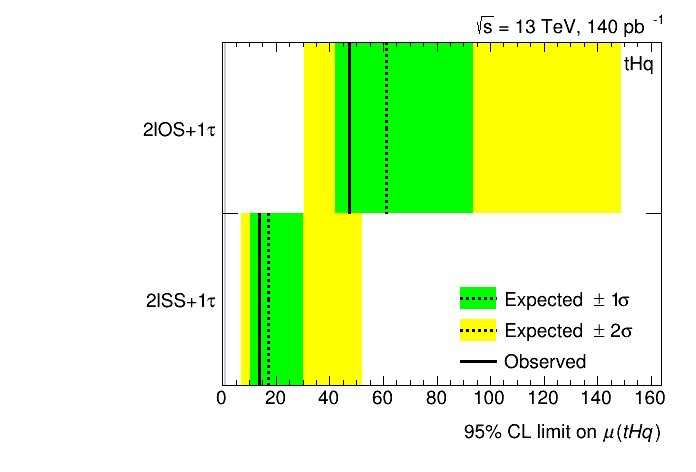
\includegraphics[width=.70\linewidth]{Chapter5_tHq/comb/Limits}
\caption{Observed and expected upper limits for the $\mu_{\tHq}$ for both \dileptau channels. The green and yellow areas represent the  $1\sigma$ ($68\%$ CL) and $2\sigma$ ($95\%$ CL) variations of the expected upper limit.}
\label{fig:Conclusion:UpperLimits}
\end{figure}


Looking ahead, the prospects for enhancing the outcomes of this analysis are promising, driven by several anticipated developments:
\begin{itemize}
	% Identificar mejor la identificación de taus es muy difícil pero lo que se podría hacer es mejorar la 
	% determinación de los fake factors (se puede hacer con más estadística o con un método mejor).
	% Nuestro sistemático dominante se debe al método de determinación de fake factors, mejorar el método
	% llevaría a reducir este sistemático.
	%\item The normalisation of fake factors\pablo{poner algo de cómo reducir el impacto de los fake taus}
	\item The upcoming high-luminosity Run 3 promises increased statistical significance of the analysis.
		This will be very beneficial since in the \dilepSStau channel (the one with the best sensitivity)
		the statistical uncertainty is the dominant. In the \dilepOStau the uncertainty due to the statistical
		sample is similar to the systematic uncertainty and more data events will undoubtedly enrich this search.

	\item The current techniques to estimate the rates of backgrounds due to misidentified objects will also
		benefit from an increase in the statistical sample since these are data-driven methods.

	\item As already mentioned, a significant challenge in the analysis presented in this thesis stems from the 
		lack of agreement observed between the actual data and the MC-event samples. 
		These discrepancies are attributed to limitations in the application of the template-fit method.
		Although the caveat in the implementation of the template is identified, a solution to it is not available at the time of composing this thesis.
		Concerning this obstacle, it may be beneficial to explore alternative methods to estimate the rates of the backgrounds based on misidentified objects.

		
	\item With more statistics we could explore splitting the regions used in the fit calculations
		according to the track multiplicity of the \tauhad (1-prong or 3-prong). %1-prong // 3-rpong
		Since jets with different origins mimic differently the \tauhad depending on its prongness,
		it can be beneficial to explore this classification when defining the regions used in
		the profiled-likelihood fit.
		%the different relative background contributions in all regions
		%considered in the fit.
		
	\item The impact of the simulated number of events for certain samples is unfortunate. 
		An improvement is expected from incorporating newer samples which have been simulated with more statistics.
		While the effect of low MC statistics could be mitigated more sensitive bins with less sensitive bins,
		after some tests, it is seen that the sensitivity of the analysis decreased by doing so.
		
	\item Currently, there is a mild tension between the simulation and the experimental results for \ttW. 
		Therefore, progress in the simulation techniques or a better understanding of these processes will
		further refine the analysis. This will be useful in the \dilepSStau channel, where this is the second
		most important background.
\end{itemize}


Additionally, this analysis can be extended in several ways.
First, the region definition can be improved by combining the BDTs described in this thesis with the NNs that are also being used by the ongoing ATLAS analysis. 
Secondly, the measurement of the \tHq production in the \dileptau channel can be combined with the measurements in other channels. 
From the two sub-channels explored in this thesis, the \dilepSStau one is the one that can add more sensitivity to future combinations with other \tHq channels. 
Finally, incorporating the \tWH processes in the signal would allow to perform a more complete \tH search and, hence, the inverted-top-Yukawa-coupling hypothesis can be properly tested. This work is currently being done, although it is not included in this thesis. The tools and methods developed to analyse the \tHq productions are the same that are employed for the inclusive \tH measurement.



%More studies to be done:
%\begin{itemize}
	%\item Comment the results using an alternative region definition based on combination of BDT and NN
	%\item Discuss using \tH instead of \tWH
	%\item Discuss further studies using the inverted \yt
	%\item Añadir más datos mejorará la precisión estadísitica de los dos canals pero, sobre todo del canal SS 
	%	donde la statdística es la principal unncertainty conn diferencia. En OS la incertidumbre estadística 
	%	es un poco mayor que la sistemàtica.
	%\item Al tener más datos también podríamos separar los \tauhad en un 1prong y 3 prong. Esto nos permite
	%	explorar nuevas técnicas de ajuste. Los 1prong y 3 prong tienen distintos tipos de fondo
	%\item Las técnicas de estimación de tau-fake-SFs también pueden mejorar al mejorar la estadística
	%\item Los resultados obtenidos para esta tesis son comparables a los de otros
	%	canales (poner resultados Jesús). A mí me sale -3.78 $\pm$ 5 y a él algo compatible en 2LSS (5,1 $\pm$ 4.8) y en el 3L (6.3 $\pm$ 7.1)
		
%\end{itemize}




%%%%%%%%%%%%%%%%%%%%%
%  Just some snipets about statistics   %
\begin{comment}
\paragraph{Comments about hypothesis rejection}\mbox{}\\
%https://arxiv.org/pdf/1007.1727.pdf
In the search for a new signal process one defines:
\begin{itemize}
	\item Null hypothesis ($H_0$):  Taking into account only the backgrounds
	\item Alternative hypothesis ($H_1$): Considering both the backgrounds and the signal
\end{itemize}
When setting limits, the model with signal-plus-background hypothesis
plays the role of $H_0$, which is tested against the background-only hypothesis, $H_1$.
The level of agreement between the data and a hypothesis $H$ is given by the $p$-value.
The $p$-value is defined as the probability, under the assumption of $H$, of finding data of 
equal or greater incompatibility with the predictions of $H$. One can regard the hypothesis 
as excluded if its $p$-value is observed below a specified threshold.

Rejecting the background-only hypothesis in a statistical sense is only part of discovering 
a new phenomenon. A widely used procedure to establish discovery (or exclusion) in particle physics is based
on a frequentist significance test using a likelihood ratio as a test statistic. In addition to
parameters of interest such as the rate (cross section) of the signal process, the signal and
background models will contain in general nuisance parameters whose values are not taken
as known a priori but rather must be fitted from the data.

Let's consider the distribution of a kinematic variable measured at the experiment. 
This distribution can be presented in a binned histogram. The expected number
of events the $i^{th}$ bin is given by:
\begin{equation*}
	n_{i}^{exp} = \mu s_{i}^{exp} + b_{i}^{exp}
\end{equation*}
Where $\mu$ is the signal strength and, if $\mu=0$ corresponds tothe background-only hypothesis .
The $s_{i}$ + $b_{i}$ are defined as:
\begin{equation*}
  s_{i}^{exp} = s_{\text{tot}}^{exp} \int_{\text{bin } i} f_s(x; \theta_s) \,dx
\end{equation*}
\begin{equation*}
  b_{i}^{exp} = b_{\text{tot}}^{exp} \int_{\text{bin } i} f_b(x; \theta_b) \,dx
\end{equation*}
The integral over $x$ runs over the kinematic distribution. The functions 
$f_s(x; \theta_s$ and $f_b(x; \theta_s)$ are the probability density functions 
(pdfs) of the variable $x$ for signal and background events.


% Bayesian vs frequentist
\paragraph{Bayesian vs frequentist}\mbox{}\\
From the frequentist point of view the probability is defined as the fraction of times an 
event occurs, in the limit of very large number ($N \to \infty$) of repeated trials
\begin{equation*}
	 \mathcal{P} = \lim_{N \to \infty} \frac{\text{Number of favorable cases}}{N}
\end{equation*}
where $N$ is the number of trials. Even though this infinity can be conceptually unpleasant, for 
LHC experiments, the amount of events is so large that this $\mathcal{P}$ definition becomes
acceptable \cite{Lista:2016chp}. 

In contrast, for the Bayesian (or subjective) probability expresses the degree of belief that a 
claim is true. Starting from a prior probability, following some observation, the probability can 
be modified into a posterior probability. The more information an individual receives, the more 
Bayesian probability is insensitive on prior probability \cite{Lista:2016chp}.

The Bayes theorem \cite{Bayes:1764vd} states that considering two events $A$ and $B$, the probability of $A$
to happen given that $B$ takes places is
\begin{equation*}
	 \mathcal{P}(A|B)= \frac{\mathcal{P}(B|A)\mathcal{P}(A)}{\mathcal{P}(B)}
\end{equation*}
where $\mathcal{P}(B|A)$ is the conditional probability of $B$ given $A$ and $\mathcal{P}(B)$ 
the probability of the event $B$ to happen. 
Here, $\mathcal{P}(A)$ has the role of prior probability while $\mathcal{P}(A|B)$ is known
as posterior probability.



\paragraph{Signal strenght}\mbox{}\\
The signal strength is defined as the ratio between the measured process
and its SM prediction. For the $\tHq$, the production signal-strength is: 
\begin{equation*}
	\mu_{\tHq} = \frac{\sigma_{\tHq}}{(\sigma_{\tHq})_{SM}} \, .
\end{equation*}
For particular decay mode $f$ its signal strength is:
\begin{equation*}
	\mu^{f} = \frac{BR^f}{(BR^f)_{SM}} \, , 
\end{equation*}
being $BR^f$ the branching ratio for the $f$ decay mode. %The subscript SM refers to the SM prediction.
Since cross-section and the BR cannot be separated without further assumptions, only the product
can measured experimentally, leading to the combined signal strength:
\begin{equation*}
	\mu_{\tHq}^{f} = \frac{\sigma_{\tHq}\cdot BR^f}{(\sigma_{\tHq})_{SM} \cdot (BR^f)_{SM}} = \mu_{\tHq} \cdot \mu^{f} \, .
\end{equation*}
In out particular case $f$ is \dilepOStau or \dilepSStau. 
\end{comment}
 


%POSTAMBLE
\begin{comment}
asdf
%\end{document}
%ENDPOSTAMBLE
\end{comment}
